%!TEX root = ../thesis.tex

% https://akhiluk.medium.com/on-why-salvor-hardin-is-simply-the-best-74948711e136
\begin{savequote}[70mm]
	To succeed, planning alone is insufficient.\\One must improvise as well.
	\qauthor{Isaac Asimov, Foundation series}
\end{savequote}

\chapter{Related work}\label{chapter:related_work}

	% https://ieeexplore.ieee.org/document/7968828
	IoT is one of the most discussed topics in both academical and industrial research, as mentioned in Section \ref{sec:trends}.
	
	By contrast, mesh networks that use wireless technologies have been researched for decades, but have yet to be put into use in large scale.
	The correct definition of a \textit{wireless mesh network}, or WMN, is ``\textit{a communications network made up of radio nodes organized in a mesh topology instead of star topology}'' \cite{wms}.	
	This particular \textit{multi-hop network}, Figure~\ref{img:multihop}, where data ``\textit{hops}'' from a node to another until it reaches its destination, can make a difference when it comes to the interconnections in the IoT world.
	It is important that ``\textit{future IoT deployments need to focus on sustainability since huge centralized data centers (Cloud Computing) have become a critical part of the infrastructure}'' \cite{7968828}.
	
	This chapter anticipates the technical one, and shows some related projects from which the project has drawn inspiration.
	At first, challenges and solutions are presented for these WMS, alongside their advantages and disadvantages.
	Below are also presented some of the projects which have been made at various levels from homemade projects, to research, to the ones already available on the market.
	
	\begin{figure}[h]
		\centering
		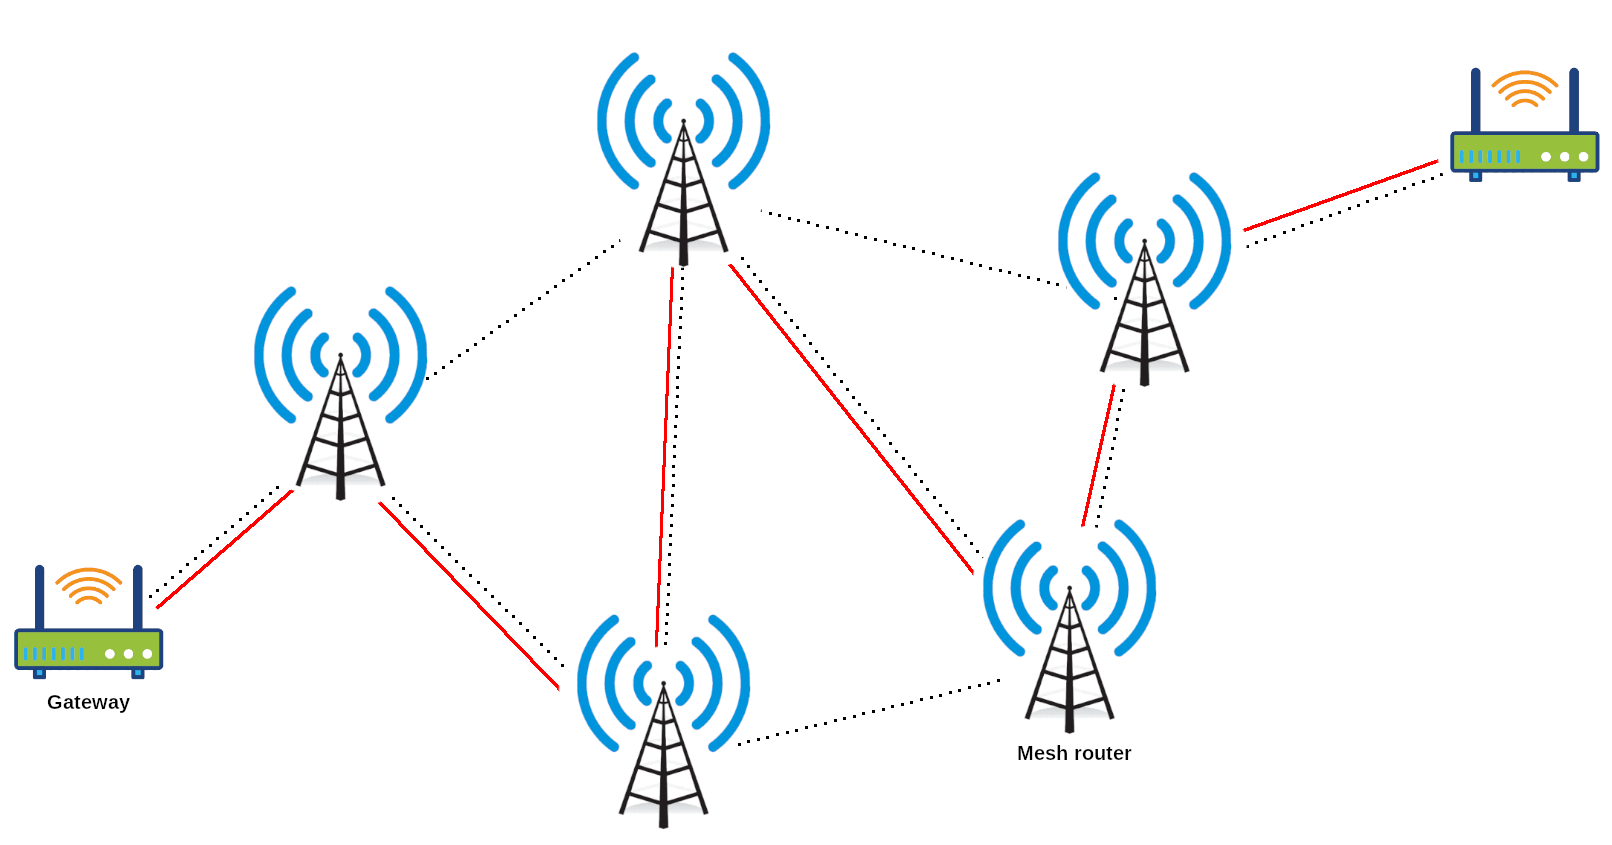
\includegraphics[width=\textwidth]{resources/img/chap4/mesh}
		\caption{Multi-hop network}
		\label{img:multihop}
	\end{figure}
	
	\section{Overview of wireless mesh networks}
		
		% https://beyondroot.com/blog/a-comprehensive-guide-to-mesh-network-in-iot-an-experts-take/		
		With new technologies, such as the ones presented in Section \ref{sec:radio_tech}, wireless mesh networking has been evolving and has reached an ideal point of maturity, which allows it to be useful in the development of IoT devices for mass production.
		Also, the rising number of connected homes and industry support on open-source resources has made mesh networking truly accessible and low-cost.
		Such networks are starting to be regarded as more viable and real choices for commercial as well as industrial IoT applications.
		Besides the possibilities such networks can bring in optimizing communication among nodes, a big advantage is the possibility of bringing connectivity in a system where nodes might have limited connection.
		
		Some of the applications for this network topology are:
		\begin{itemize}
			\item \textit{smart cities}: extending radio signals through campus grounds, business parks, parking garages, and other outdoor facilities;
			\item \textit{healthcare equipment}: monitoring and locating medical equipment, also serve as a backup for medical devices that always require to stay online;
			\item \textit{smart home}: track and manage data from sensors all around the house;
			\item \textit{farming}: in areas where power and connectivity are highly limited, mesh networking is ideal to track sun exposure and water levels across the crops and fields, for example.
		\end{itemize}
	
		Before choosing a mesh network topology it is important to evaluate aspects such as \textit{installation}, \textit{device management} and \textit{support}.
	
		\textit{Energy management} represents an important factor as well, since the connected devices could be small battery operated.
		Thus, efficient transmission techniques and protocols that consider the amount of energy used, must be developed in order to optimally use the batteries on such devices		
		That is why there is a particular network topology, \textit{Low Power Wireless Area Network}, focused on the interconnection of these devices, described in Section \ref{sec:radio_tech}.
		
		Solutions to optimize the networks can be implemented both via hardware, via repeaters, and software.
		% https://ieeexplore.ieee.org/document/4068249
		The latter is mainly implemented with with AI techniques, which allow protocols to ``\textit{learn}'' how to spatially coordinate and adapt contention patterns.
		Authors of \cite{4068249}, for example, have developed new distributed MAC scheduling algorithms by combining synchronous two-level priority RTS/CTS\footnote{ \textit{Request To Send / Clear To Send}} handshaking with randomized time slot selection.
		From these ``\textit{adaptively biasing time-slot selection probabilities based on past history, one can develop variations that are also provably throughput-optimal and exhibit better convergence rates}''.
		
		% https://ieeexplore.ieee.org/document/7968828
		Classic network topologies, such as the ones in Figure~\ref{img:network_topologies}, are not designed for IoT communication and might not be able to meet the requirements for such, and more, dynamic devices, which are also low-powered sensors.
		Another important setback of such networks is their single point of failure nature, which ``\textit{makes the entire system extremely vulnerable when it comes to disasters or even difficult environment as the sensors may need to be deployed into some hardly reachable locations}'' \cite{7968828}.
		
		An example of a multi-hop wireless mesh network is \textit{VANET} (\textit{Vehicular Ad-Hoc Network}), a particular case of wireless multi-hop network, which has the constraint of fast topology changes due to the high node mobility, Figure~\ref{img:vanet}.
		
		\noindent
		\begin{minipage}{0.52\textwidth}
			\begin{figure}[H]
				\centering
				\includegraphics[width=\textwidth]{resources/img/chap4/wms_microsoft}
				\caption[Self organizing wireless mesh networks]{Self organizing wireless mesh networks \cite{bahl2009opportunistic}}
				\label{img:wms_microsoft}
			\end{figure}
		\end{minipage}%
		\hfill%
		\begin{minipage}{0.48\textwidth}\raggedright
			\begin{figure}[H]
				\centering
				\includegraphics[width=\textwidth]{resources/img/chap4/vanet}
				\caption[An example of a VANET]{An example of a VANET \cite{BADIS2015653}}
				\label{img:vanet}
			\end{figure}
		\end{minipage}
		\newline
		
		This is a very important type of network, giving the increasing number of vehicles equipped with computing technologies and wireless communication devices.
		Authors of \cite{BADIS2015653} explain how such increase ``\textit{intervehicle communication is becoming a promising field of research, standardization, and development}''.
		A tangible example can be seen in the rising of electric vehicles and their constant rise in sells on the market, which brought more attention on the aforementioned factors.
		
		Microsoft has also tried to apply mesh networking to normal Internet household use \cite{bahl2009opportunistic}, however, given the improvements in telecommunication infrastructures and the advancement of fiber optics and Internet via cable, the project has been abandoned.
		Their proposed topology is represented in Figure~\ref{img:wms_microsoft}
		This shows how each network topology is better suited for particular scenarios.
		
		Compared to the example of Microsoft's project, a VANET is more suited for a wms since the data transfered among cars is less than the one transfered among houses.
				
		% BLUETOOTH
		% https://www.ericsson.com/en/reports-and-papers/white-papers/bluetooth-mesh-networking
		
		% https://beyondroot.com/blog/a-comprehensive-guide-to-mesh-network-in-iot-an-experts-take/
		The components of a mesh network usually are:
		\begin{itemize}
			\item \textit{nodes}: devices that communicate data with each other;
			\item \textit{gateway}: allows devices to transfer data in the network, also provides a backhaul to the Internet for the local mesh network;
			\item \textit{repeater}: repeaters that maintain signal and forward messages between endpoints
			\item \textit{endpoint}: mesh-only devices that don't route messages for other devices, but send them to other nodes.
		\end{itemize}
		\vspace*{-\baselineskip}
		
		% TODO CHECKED UNTIL HERE
		\subsection{Advantages of WMS}
		
			% https://beyondroot.com/blog/a-comprehensive-guide-to-mesh-network-in-iot-an-experts-take/
			Mesh Network for IoT devices offers enormous benefits that make it sought-after in enterprises and significant in an IoT app development company.
			Self-healing
			
			Like Shortest Path Bridging, Self-healing algorithm automatically chooses the best path to transfer data even if a few nodes lose connection. Specifically, it uses only those connections that are available and working to maintain the task.
			Self-configuring
			
			Due to auto-discovery, mesh networks are self-configuring in nature. Hence, the new nodes calibrate automatically and connect to the network without any previous setup. Consequently, network administration and expansion become easier in mesh networking.
			Scalability and Reliability
			
			In a mesh network, it is way easy to add or remove nodes without any efficiency issue. Usually, issues are in proportion to the devices. However, it is quite the opposite in the case of a mesh network. Adding nodes in a mesh network provides more routes in which data package can travel, which makes the network faster, reliable, and error-resistant.
			Cost Reduction
			
			Since mesh networks do not require internet connection, it consumes ultra-little energy. Meanwhile, sensors are pocket-friendly and long-lasting.
			
			Besides, IoT implementation reduces expenses in many other ways like better management, optimization of resources usage, and more.
		
		\subsection{Disasvantages of WMS}
		
			Drawbacks of Mesh Network in IoT
			
			Though there are ample benefits of a mesh network, it also comes with a few drawbacks. So, it is essential to gain in-depth knowledge of this network before deciding whether a mesh network is a perfect fit for you.
			Low Capacity
			
			Mesh network is the best way of sending small data packages. Unfortunately, it doesn’t perform well while transferring video file sized data.
			
			Still, if transferring a large amount of data is compulsory, then the Wi-Fi mesh network would be a better option.
			Latency
			
			Actively switching from one node to another can decelerate the data receiving process. However, it is not an issue when your system requires a package every few minutes or so. But, it might be not enough for a few systems.
			
			Conversely, a full mesh network can accelerate the data transfer by connecting every node to one another.
			Maintenance
			
			Due to the self-healing ability of the mesh network, finding a non-working node might be time-consuming. Also, we won’t come to know if a node is having an issue.
			
			On the other hand, mesh networks for IoT devices are established to make the IoT system smarter and more efficient. So, the nodes are less prone to crash.
		
			% https://www.inthemesh.com/archive/the-scalability-of-mesh-networks/\\
			
			% https://ieeexplore.ieee.org/document/8071545
			
			% PAPER: LoRaWAN Range Extender for Industrial IoT
	
	\section{Algorithms for lora Wireless Mesh networks}
	
		% https://www.springerprofessional.de/en/research-on-using-the-aodv-protocol-for-a-lora-mesh-network/18715992
	
	\section{Projects}\label{sec:chap4_projects}
		
		Here are three categories of projects:
		
		\subsection{Open source projects}
		
			% https://www.hackster.io/scottpowell69/lora-mesh-chat-5267d9
			\subsubsection{LoRa Mesh Chat}\label{subsubsec:lorameshchat}

				This project consist in an add-on for mobile phones that enable text messaging in a group when outside cellular and Internet coverage.		
					
				\noindent
				\begin{minipage}{0.5\textwidth}% adapt widths of minipages to your needs
					\begin{figure}[H]
						\centering
						\includegraphics[width=.8\textwidth]{resources/img/chap4/lora-mesh-chat-5267d9}
						\caption{ESP32 Lora with OLED}
						\label{img:lora_mesh_chat}
					\end{figure}
				\end{minipage}%
				\hfill%
				\begin{minipage}{0.5\textwidth}\raggedright			
					As explained on the project's webpage \footnotemark, an ESP32 microcontroller with a LoRa antenna and an OLED display is programmed to connect to the phone either via and OTG cable or BLE.
					By using an application on the phone, the user is capable of sending text messages in a group.
				\end{minipage}			
				\footnotetext{{ \url{www.hackster.io/scottpowell69/lora-mesh-chat-5267d9}}}
				
				\subsubsection{Meshtastic}\label{subsubsec:meshtastic}
	
					% https://meshtastic.org/
					% https://github.com/meshtastic
					% https://www.hackster.io/punkgeek/meshtastic-a-hiking-skiing-gps-mesh-communicator-84f999
						
					Meshtastic is an open-source hiking, pilot, skiing, Signal app-extending GPS mesh communicator.
					
					Meshtastic is a project that lets you use inexpensive (\$30 ish) GPS radios as an extensible, super long battery life mesh GPS communicator. These radios are great for hiking, skiing, paragliding - essentially any hobby where you don’t have reliable internet access. Each member of your private mesh can always see the location and distance of all other members and any text messages sent to your group chat.
					
					The radios automatically create a mesh to forward packets as needed, so everyone in the group can receive messages from even the furthest member. The radios will optionally work with your phone, but no phone is required.Our device code is here, our optional Android app is here.
					
					Prebuilt binaries are included on the github sites, but it is quite easy to build from source. Instructions are included in the README. No soldering is required, essentially - buy a \$30 radio and go. We'd love to have your help extending the project - it has been super fun to work on.
		
		\subsection{Research projects}
		
			\subsubsection{Monitoring of Large-Area IoT Sensors Using LoRa Wireless Mesh Network System: Design and Evaluation}
			
			\subsubsection{Black Powder Flow Monitoring in Pipelines by Means of Multi-Hop LoRa Networks}
		
			\subsubsection{Exploring Multi-Hop LoRa for Green Smart Cities}
			
			\subsubsection{Proposal of a Hybrid LoRa Mesh / LoRaWAN Network}
			
			\subsubsection{Beyond the Star of Stars: An Introduction to Multihop and Mesh for LoRa and LoRaWAN}
			
			\subsubsection{LoRa-based Mesh Network for Off-grid Emergency Communications}
			
			% https://ieeexplore.ieee.org/document/9394317
			\subsubsection{LoRaCTP}
			
				a flexible protocol based
				on LoRa technology that allows for the transfer of “content” to
				large distances with very low energy. LoRaCTP provides all the
				necessary mechanisms to make LoRa reliable, by introducing a
				lightweight connection set-up and ideally allowing the sending
				of an as-long-as necessary data message.
			
				\begin{figure}[H]
					\centering
					\includegraphics[width=.75\textwidth]{resources/img/chap4/loractp_packet}
					\caption[Flow of the establishment and interchange of data in LoRaCTP]{Structure of the packet used by the stop-and-wait ARQ. \cite{loractp}}
				\end{figure}
			
				\begin{figure}[H]
					\centering
					\includegraphics[width=.5\textwidth]{resources/img/chap4/loractp_flow}
					\caption[Flow of the establishment and interchange of data in LoRaCTP]{Flow of the establishment and interchange of data in LoRaCTP \cite{loractp}}
				\end{figure}
		
		By content we refer to a self-contained piece of data, like a
		JSON encoded message whose length is in principle unlimited.
		We tested out library with messages of up to 150 kbytes,
		as indicated in Section V. LoRaCTP is based on a unicast
		protocol adopting a classical stop-and-wait ARQ approach
		with a dynamic and adaptive value for the retransmission
		delay. The protocol ensures that information is not lost due to
		dropped packets and that packets are received in the correct
		order.
		
		Each packet is sent by using a three attempts scheme. That
		is, if after three attempts no ACK is received, we suppose
		that the channel is currently busy or too noisy and the content
		sending is dropped.
		
		On top of this flow-control protocol there is a lightweight
		transport protocol that is used to establish a connection be-
		tween a master node, and a client node. Figure 3 shows a sim-
		ple sequence example. Basically the master device “listens”
		to incoming connections. Connections can be established in a
		unicast manner, by providing the address of the master device,
		or using an anycast approach, thus sending to the generic
		“00000000” address and thus receiving the reply from the
		close-by listening device. This possibility allows for a greater
		flexibility in establishing dynamic topologys in rural areas, for
		example.
		
		% https://www.project-owl.com/
		% https://www.reddit.com/r/RTLSDR/comments/bzian5/ltt_showcases_new_lora_mesh_network_devices/

		% TODO DONE CHECK FROM HERE ON
		\subsection{Commercial applications}

			% SONNET
			% https://www.kickstarter.com/projects/sonnet/sonnet-decentralized-mobile-communication
			% https://www.indiegogo.com/projects/sonnet-game-changer-for-wilderness-communications#/
			% GOTENNA
			% https://gotenna.com/
			%				https://gotennamesh.com/products/mesh?utm_source=internal-link&utm_medium=menu&utm_campaign=gotenna.com
			% https://techcrunch.com/2019/06/18/gotenna-is-ramping-up-public-sector-mesh-networking-with-a-24m-c-round/
			\subsubsection{Off grid mesh devices: Sonnet and goTenna}
			
				Both of the following devices use LoRa to create a mesh network and have been designed for emergency off-grid communication, where cellular towers or land-line phones are not physically reachable.
				
				\begin{minipage}{0.38\textwidth}% adapt widths of minipages to your needs
					\begin{figure}[H]
						\centering
						\includegraphics[width=.8\textwidth]{resources/img/chap4/sonnet}
						\caption{Sonnet}
						\label{img:sonnet}
					\end{figure}
				\end{minipage}%
				\hfill%
				\begin{minipage}{0.62\textwidth}\raggedright
					Sonnet\footnotemark, in Figure~\ref{img:sonnet}, connects to the smartphone via Wi-Fi allowing the user to send texts, voice messages, images, data, files and share GPS locations to any other Sonnet users up to several kilometers away, thanks to LoRa.
					This completely removes smartphones' dependency on cellular grid and other network infrastructure, and allows Sonnet to be used even when there is no cellular connectivity or Internet access.
				\end{minipage}		
				\footnotetext{~\url{www.sonnettech.com}}
			
				According to the product's Kickstarter page\footnote{ \url{www.kickstarter.com/profile/sonnet/created}} ``\textit{with Sonnet, data can be relayed up to 16 times to achieve a maximum range of 80 km (50 miles)}''.

				\begin{minipage}{0.5\textwidth}%
					\begin{figure}[H]
						\centering
						\includegraphics[height=6cm]{resources/img/chap4/gotenna}
						\caption{goTenna Mesh}
						\label{img:gotenna}
					\end{figure}
				\end{minipage}%
				\hfill%
				\begin{minipage}{0.5\textwidth}\raggedright
					\begin{figure}[H]
						\centering
						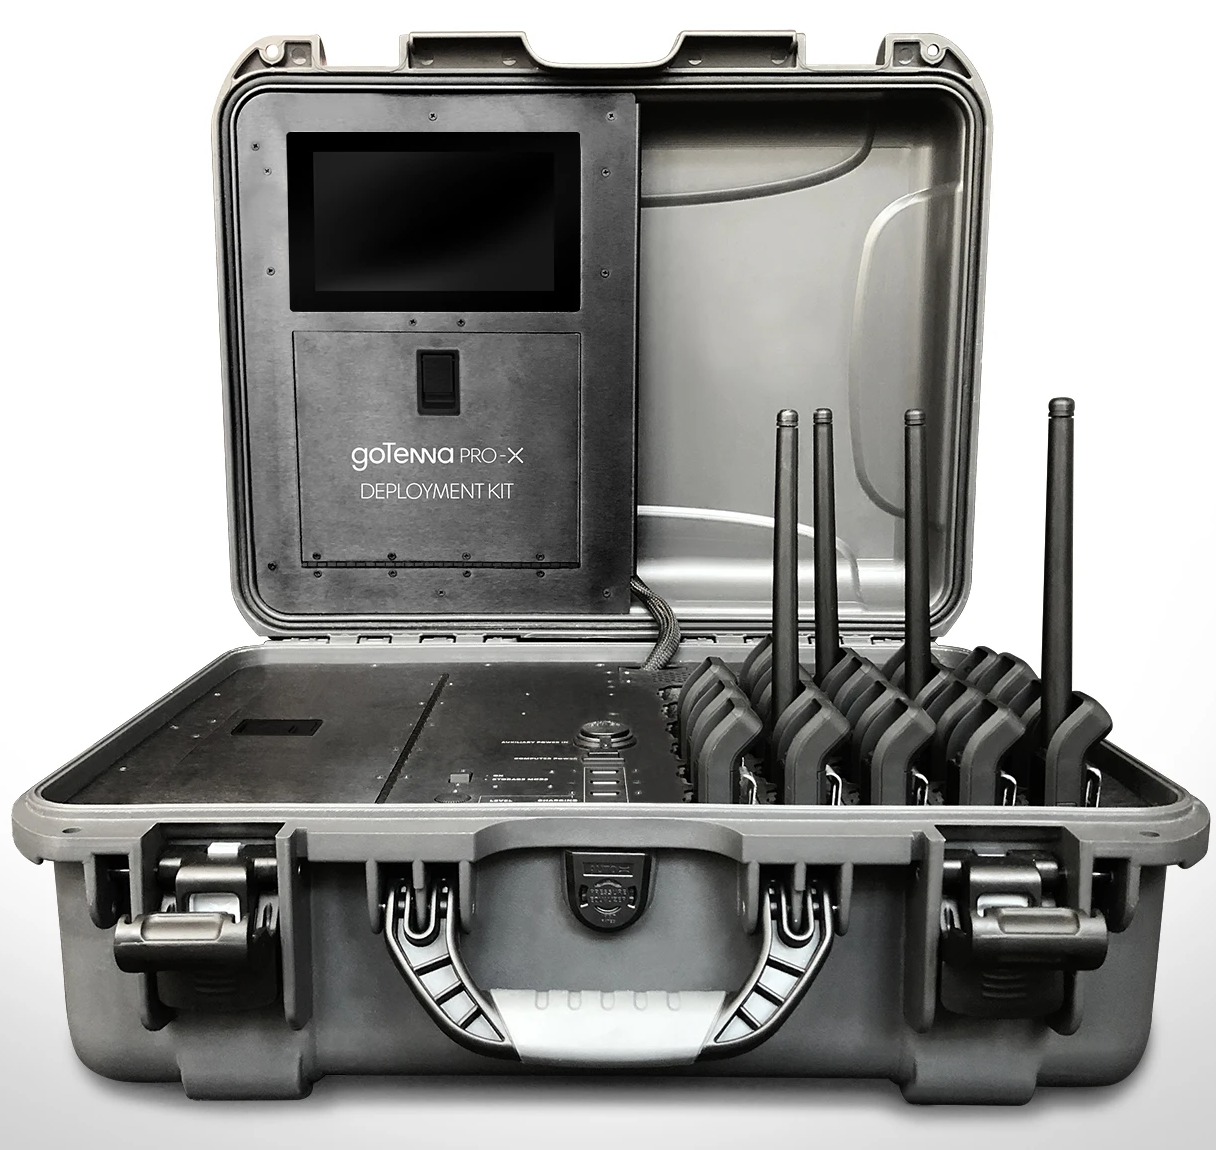
\includegraphics[width=.9\textwidth]{resources/img/chap4/gotenna_prox}
						\caption{goTenna Pro}
						\label{img:gotenna_pro}
					\end{figure}
				\end{minipage}%
				\newpage
				
				The goTenna\footnote{ \url{www.gotenna.com}}, in Figure~\ref{img:gotenna}, offers similar functions as the Sonnet, allowing to send text and GPS locations without the use of a cellphone with Internet connectivity.
				Mesh-networking allows to relay messages from a node to another until they reach destination.
				
				A compact and ruggedized kit, the goTenna Pro X, in Figure~\ref{img:gotenna_pro}, allows control for larger teams that operate in complex environments where it is not possible to be offline.
						
				As Sonnet, goTenna has raised the funds necessary to enter the market as a crowdfunded project on Kickstarter\footnote{ \url{www.kickstarter.com/profile/gotenna/created}}.
				
				Compared to the projects in Section \ref{subsubsec:lorameshchat} and Section \ref{subsubsec:meshtastic}, Sonnet and goTenna offer a more stable network, thanks to the fact that they can be considered finished products which have been thoroughly tested and produced on a bigger scale.
						
			% https://www.linksys.com/us/r/resource-center/whole-home-mesh-Wi-Fi/
			% https://www.pcmag.com/picks/the-best-wi-fi-mesh-network-systems
			\subsubsection{Mesh Wi-Fi}
					
				\textit{Mesh Wi-Fi}, or \textit{Whole Home Wi-Fi} systems, consists of a main router that connects directly to the main modem, and a series of satellite modules, or nodes, placed around the house for full Wi-Fi coverage.
				Each node serves as a hop point for other nodes in the system and are all part of a single wireless network and share the same SSID and password, unlike traditional Wi-Fi routers.
				Weakened signal or Wi-Fi dead spots of the latter are the result of physical obstructions (floor, doors, and walls).
				
				A modular mesh whole home Wi-Fi system is flexible and scalable, giving a customizable method of expanding Wi-Fi coverage without the need to add range extenders, which are certainly effective when it comes to increasing the router range, but they do so at the expense of Wi-Fi performance, which gets cut in half.
			
				\begin{figure}
					\centering
					\includegraphics[width=.9\textwidth]{resources/img/chap4/wifi6}
					\caption{Wi-Fi 6 mesh nodes compared to Wi-Fi range extenders performance}
					\label{img:Wi-Fi6}
				\end{figure}
				
				Wi-Fi 6 is an evolution of 802.11ac technology, which promises increased throughput speeds (up to 9.6Gbps), less network congestion, greater client capacity, and better range performance thanks to the improved wireless technologies, including \textit{Orthogonal Frequency-Division Multiple Access} (\textit{OFDMA}).
				The latter improves overall throughput by breaking Wi-Fi channels into sub-channels, allowing up to 30 users to share a channel at the same time.
				
				Many important manufacturers for network hardware, like Netgear and Cisco, have already implemented such technology and functions in their products available not only for industrial purposes, but also for average users.
				